\documentclass[a4paper,12pt]{article}

\usepackage[portuguese]{babel}
\usepackage[T1]{fontenc}
\usepackage[utf8]{inputenc}
\usepackage{hyperref}
\usepackage{graphicx}
\usepackage{float}
%\usepackage{multirow}
\usepackage[hypcap]{caption} % makes \ref point to top of figures and tables
\usepackage{amsmath}
%\usepackage[usenames,dvipsnames,svgnames,table]{xcolor}
%\usepackage{rotating}
\usepackage[margin=0.95	in]{geometry} %margens da página


\begin{document}

	\pagenumbering{gobble}
	\begin{titlepage}

	\begin{center}

		
\includegraphics[width=6cm]{img/tecnico_logo}\\[3cm]

		\textsc{\LARGE Sistemas Computacionais Embebidos}\\[1.5cm]

		\Large 1ª Parte\\[1.5cm]


		{ \huge \bfseries Sistema de Monitorização e Alarme\\[2.5cm] }


		\noindent
		\begin{center} \large
			Francisco Leal, 72939\\[5mm]		
		
			Gonçalo Ribeiro, 73294\\[5mm]

			Ricardo Amendoeira, 73373\\[2.5mm]
			
			\vfill

			\textit{Docente: Prof. Carlos Almeida}\\[1cm]

		\end{center}

		{\large \today}

	\end{center}

\end{titlepage}

	\tableofcontents
	\pagebreak
	
	\pagenumbering{arabic}

\section{Fluxograma}



\begin{figure}[H]
\centering
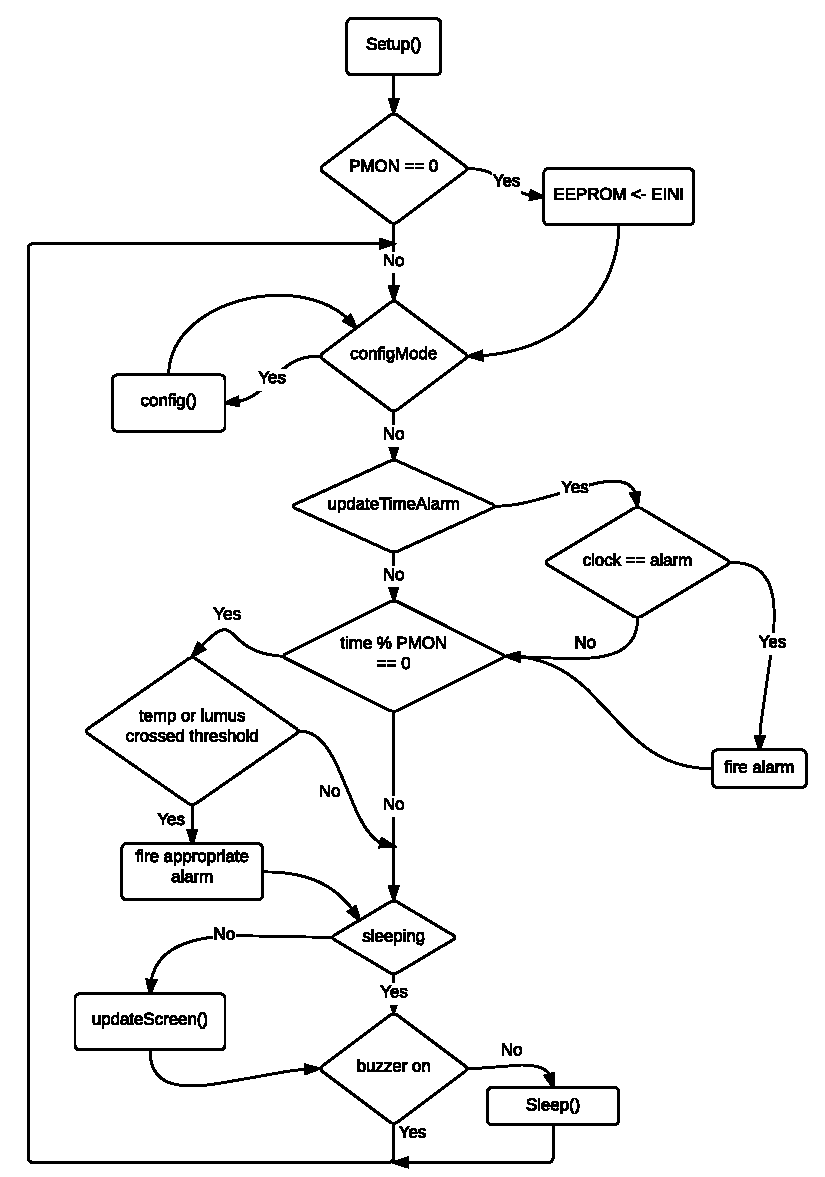
\includegraphics[width=.9\textwidth]{img/flowchart.pdf}
%\caption{}
\end{figure}

\pagebreak

\section{Estruturas de Dados}

\subsection{Buffer Circular}

Os registos armazenados estão alinhados a 8 bytes, de modo a que não haja escritas distribuídas por duas páginas. Assim pode-se sempre escrever 8 bytes de uma vez, sem nunca ter que verificar se é necessário continuar a escrever noutra página. Os últimos 8 endereços estão reservados para guardar a informação necessária à manutenção do buffer circular. Para endereçar a EEPROM externa é necessário enviar 2 bytes de endereço através do protocolo I$^2$C, visto que a EEPROM tem 32K $\times$ 8 bits.

\subsection{Tempo}

Para o controlo do relógio e do alarme foi definida uma estrutura que contém os segundos, minutos e horas, cada um guardado como um byte. A interrupção do Timer1 actualiza a cada segundo a estrutura que guarda o tempo. Outros eventos que podem ocorrer apenas em tempos múltiplos de um segundo são também sinalizados por esta rotina de interrupção.

\subsection{Configuração}

No modo configuração é possível ligar e desligar os alarmes individualmente e assim alterar os vários valores que são configuráveis (clock, alarm, limiar de temperatura e de luminosidade), por exemplo, é possível ligar apenas o alarme da temperatura e não ligar os restantes alarmes.


\section{Rotinas}

\subsection{\texttt{Config()}}

Quando em modo normal, se pressiona o botão S3 uma interrupção é chamada que activa/altera o modo de configuração. Dentro do \texttt{config()} entra-se em modo de configuração e o programa mantêm-se nesse modo até que se tenha passado por todos os parâmetros que podem ser configurados -- tempo, alarme, limiar de temperatura e luminosidade. O botão S3 permite portanto seleccionar o parâmetro a alterar, enquanto que o botão S2 permite alterar o valor seleccionado.

Foi implementado \textit{debounce} para o botão S2, de forma a que cada vez que se carrega neste botão, o valor que está a ser alterado seja incrementado em apenas uma unidade. Não foi implementado \textit{debounce} para o botão S3 visto que este tem um schmidtt trigger à entrada, o que resolve o \textit{bounce} neste botão.

De modo a minimizar o consumo energético é registado que parâmetros são alterados de modo a apenas actualizar no ecrã e em memória os valores que realmente foram redefinidos pelo utilizador.

\subsection{Alarmes}

Os alarmes de luminosidade e temperatura têm período de amostragem \texttt{PMON}. Se os limiares de temperatura ou de luminosidade forem cruzados (em qualquer sentido), o respectivo alarme dispara. Para fazer a verificação é mantido em memória o valor da amostra anterior.
A verificação do alarme do relógio é feita de segundo em segundo. Antes de serem efectuadas comparações, as interrupções são desligadas para garantir a consistência destas.

\subsection{Interrupções -- Timer1, S3, WREN e LVD}

A interrupção do Timer1 é chamada de segundo a segundo e actualiza a hora do relógio. Nesta interrupção também é verificado se já passaram \texttt{PMON} segundos desde a última verificação e é preciso voltar a verificar os valores dos vários alarmes.

A rotina de interrupção \texttt{S3\_isr()} é invocada sempre que se utiliza o botão de pressão S3, que altera o campo selecionado no modo configuração.

A rotina \texttt{LVD\_isr()} é invocada quando é detectada uma queda na tensão de alimentação. Através de variados testes não foi possível registar na EEPROM interna mais do que um byte pelo que foi tomada a decisão de registar os minutos, as horas e os valores de limiar para os alarmes de temperatura e luminosidade sempre que estes são alterados. Desta forma, apenas temos que registar o valor dos segundos quando a rotina \texttt{LVD\_isr()} é chamada.

De modo a saber se o que foi registado na EEPROM interna é válido ou não, um valor predefinido de \texttt{0xFF} é colocado na posição destinada ao campo dos segundos no início da execução do programa. Se ao iniciar o programa o valor que estiver nesta posição de memória não for um valor válido para o campo dos segundos então é porque a interrupção LVD não teve tempo de escrever na EEPROM interna. Neste caso o relógio é iniciado a \texttt{00:00:00}.

Os limiares dos alarmes de temperatura, luminosidade e alarme são inicializados a 0, a não ser que o checksum destes dados esteja correcto. O \textit{checksum} é a soma dos valores anteriormente referidos.

A rotina \texttt{EEwriteDisable\_isr()} é invocada quando a escrita que está a decorrer para a EEPROM interna acaba. Esta rotina faz \textit{disable} à escrita para a EEPROM interna.

\end{document}
